\documentclass[12pt,a4paper]{article}
\usepackage[margin=2cm]{geometry}
\usepackage{graphicx}
\parskip = 12pt
\parindent = 0pt
\linespread{2}
%begin{XeTeX}
\usepackage{fontspec}
\setromanfont{AR PL New Kai}
\setmonofont{AR PL New Sung Mono}
\XeTeXlinebreaklocale "zh"
\XeTeXlinebreakskip = 0pt plus 1pt
%end{XeTeX}
\begin{document}

\begin{titlepage}

\begin{center}

\begin{Large}
教育部主辦\\[1cm]
九十七學年度大學校院\\[1cm]
積體電路電腦輔助設計軟體製作競賽\\[1cm]
競 賽 報 告
\end{Large}

\vfill

\begin{large}
組  員:941522 游竣彥\\
     941540 陳弘逸
\end{large}

\vfill

\begin{Large}
Failure Candidate Identification for Silicon Debug
\end{Large}

\vfill

\begin{large}
中華民國九十七年 12 月 28 日
\end{large}

\end{center}

\end{titlepage}



\section{Abstract}

  在第一個 silicon prototype 被大量製造以前,首要的事情就是確認製造%
的過程和系統的整合,而下圖表示在 silicon prototype 被大量製造以前,%
silicon 所要作的測試。

\begin{center}
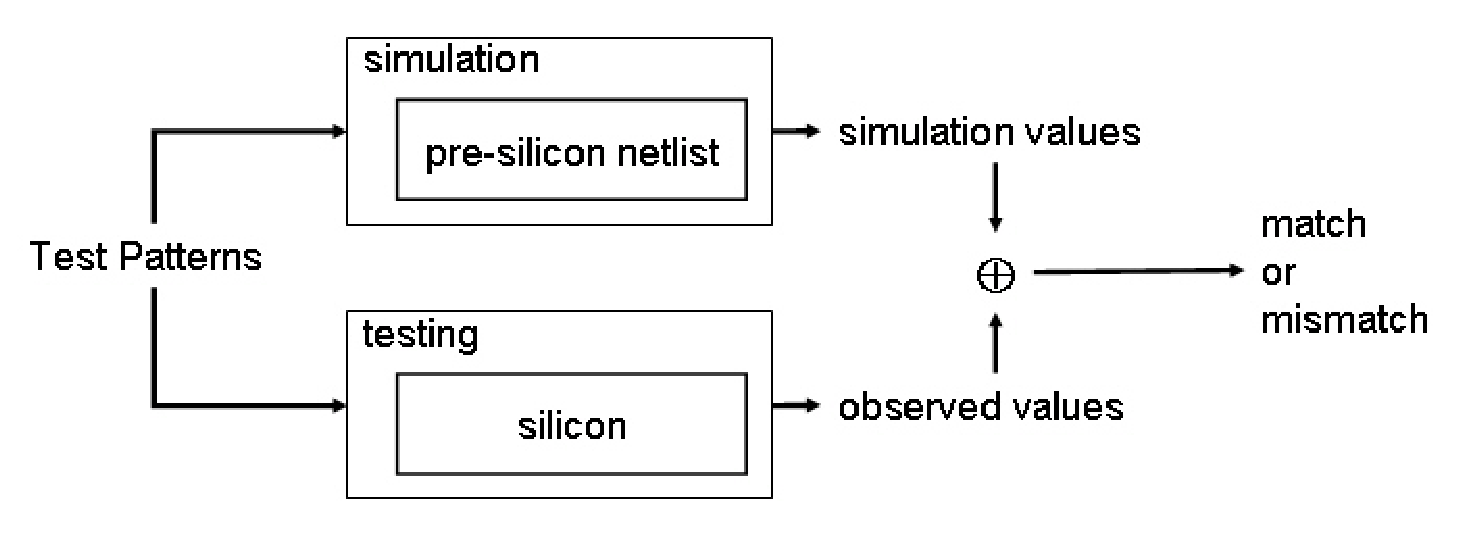
\includegraphics[scale=0.6]{imgs/01.eps}
\end{center}

  當我們拿到 test pattern 後,我們會做兩種測試,分別為 simulation %
和 testing ,如果兩種測試出來的結果相同,則就是 match,不同的話則是%
mismatch,而我們所做的程式,則是在得到 mismatch 後,對於 silicon %
prototype 做 debug,找出裡面的有可能的 defective signal。

\section{Introduction}

\subsection{Problem Description}

  給予以下三個 input 檔案:

\begin{enumerate}
\item verilog 的 pre-silicon flatten gate-level netlist。
\item silicon 作 simulation 所有 signal 的 dump value。
\item silicon 做 testing 最後所得到的 output value。
\end{enumerate}

我們要做 debug,找出有可能的 defective signal。

  為了能找出 mismatch behavior,我們使用 What–if 這個方法,%
藉由改變目前的 value,我們可以快速的找出問題所在,在這裡,我們只討論%
一次改變一個 signal。以下圖的 n2 為例,我們將 n2 的 1 改變為 0,則 O1、%
n4 和 O2 的 value 皆會改變,如果改變後的 output 與 testing 觀察所得到%
的 value 一樣的話,那麼 n2 可能就是一個 defective signal。

\begin{center}
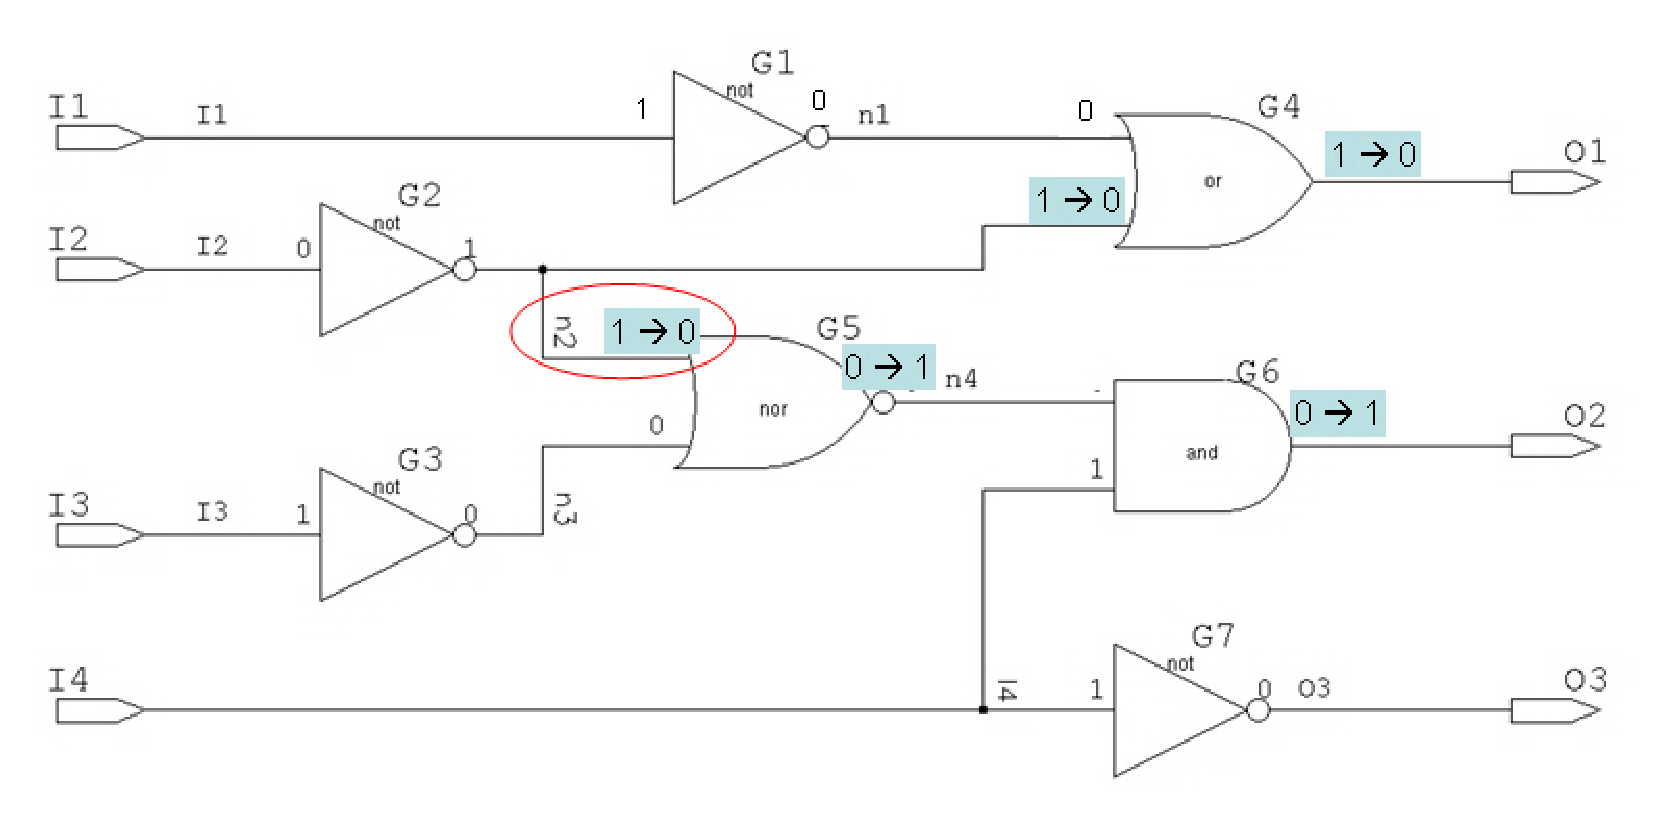
\includegraphics[scale=0.6]{imgs/02.eps}
\end{center}

    因此,我們需要一個程式,能夠將所有有可能的 defective signal 給%
找出來,並且利用一些演算法,找出有可能是 defective signal 的 signal,%
在對這些 signal 做 What–if 分析,如此一來,可以減少很多不必要%
的 What–if 分析,已達到 debug 最大的效率。

\subsection{Functions and Features}

  本軟體依照上述的需求,完成所應該要做的分析,並且利用%
兩個演算法,減少不必要的 What-if 分析,在最短的時間內%
把有作 What–if 的 signal 和最後有可能的 defective signal 給列出來。%

\subsection{Contributions and Results}

  為了減少不必要的 What–if 分析,我們依照題目的提示%
設計了兩個演算法,分別為 Static approach 和 Dynamic approach,%
利用這兩種演算法,我們便可以提升程式的效率。

\section{Algorithms}

\section{Implementation}

\end{document}
